\chapter{Special Relativity: Reference Frames, Light, and Spacetime}

This quarter returns to classical physics, but now at its relativistic end. We have already learned the structure of Newtonian mechanics, and we have seen enough quantum mechanics to know that more will be needed later, but not yet. The next real subject is light, and light forces us to rethink space and time themselves. These notes follow Leonard Susskind's first lecture in the 2012 spring \emph{Theoretical Minimum} course on special relativity, with the board sequence and the lecture rhythm preserved, and with supporting lecture captures curated through LazyingArt LLC and Video2Book.

\section{Why Begin Again?}

Susskind begins by deliberately starting over. Nearly everyone in the room has seen special relativity before, but that is not a reason to skip it; it is a reason to rebuild it carefully. The payoff is that every later formula will come with its own motivation.

Before relativity in Einstein's sense, we need the older language of reference frames.

\begin{definition}
A reference frame is a coordinate system for space and time. Concretely, we imagine space filled with a lattice of meter sticks, so that every point can be assigned coordinates \(x,y,z\), together with a synchronized collection of clocks that assign a time coordinate \(t\). An inertial reference frame is one in which force-free particles move with uniform velocity.
\end{definition}

Two inertial observers assign different coordinates to the same event if they move relative to one another. They may disagree about position for obvious reasons. In pre-relativistic physics they were also assumed to agree about time. One simply wrote
\begin{equation}
t'=t,
\end{equation}
as if moving clocks and resting clocks were governed by the same universal simultaneity.

The older principle of relativity already belonged to Newtonian mechanics: the laws of physics are the same in all inertial reference frames. One may picture the standard railroad train. If we are sealed inside a train moving with uniform velocity, and we juggle or drop objects, the laws we infer are exactly the same laws we would infer at rest. Uniform motion does not announce itself from within.

Einstein adds one further law of physics: light moves with speed \(c\). Once we combine that statement with the older principle of relativity, the puzzle is immediate. If the laws are the same in every inertial frame, and the speed of light is one of those laws, then every inertial observer must assign the same speed \(c\) to light. That is where the lecture really begins.

\section{The First Puzzle: Light and the Failure of the Galilean Rule}

For the moment, we throw away two spatial dimensions and keep only one. We draw an \(x\)-axis and a \(t\)-axis, and we insist on being almost pedantic.

\begin{figure}
\centering

\includegraphics[width=0.72\textwidth]{lecture_01_figure_02.png}
\caption{Spacetime axes as the light trajectory is introduced. The equation is only partially visible on the board; the completed form comes from the transcript.}
\end{figure}

In the stationary frame, a light ray emitted from the origin follows
\begin{equation}
x=ct.
\end{equation}
On an \(x\)-\(t\) diagram this is a straight line.

\begin{figure}
\centering
\begin{tikzpicture}[scale=0.95]
\draw[->] (0,0) -- (5.7,0) node[right] {$x$};
\draw[->] (0,0) -- (0,4.7) node[above] {$t$};
\draw[thick] (0,0) -- (5.0,3.0);
\node at (4.4,2.5) {$x=ct$};
\end{tikzpicture}
\caption{A clean redraw of the first spacetime picture. The light ray is straight, with slope fixed by the speed \(c\).}
\end{figure}

Now add a second observer moving uniformly to the right. In the unprimed coordinates, that observer's world line is
\begin{equation}
x=vt.
\end{equation}
From the moving observer's own point of view, this same line is simply \(x'=0\).

\begin{figure}
\centering

\includegraphics[width=0.72\textwidth]{lecture_01_figure_03.png}
\caption{The moving observer's world line \(x=vt\), drawn against the light trajectory. The green line is interpreted from context as the light ray.}
\end{figure}

\begin{figure}
\centering
\begin{tikzpicture}[scale=0.95]
\draw[->] (0,0) -- (5.7,0) node[right] {$x$};
\draw[->] (0,0) -- (0,5.2) node[above] {$t$};
\draw[thick] (0,0) -- (5.0,3.0);
\draw[thick] (0,0) -- (2.3,5.0);
\node at (4.4,2.6) {$x=ct$};
\node at (2.6,4.6) {$x=vt$};
\node at (1.6,3.3) {$x'=0$};
\end{tikzpicture}
\caption{Light and an ordinary world line on the same \(x\)-\(t\) plane. Since \(v<c\), the world line is steeper than the light ray.}
\end{figure}

If we use the Galilean rule, the relation between the two frames is
\begin{equation}
x'=x-vt,\qquad t'=t.
\end{equation}
Now apply it to the light ray. Along the light trajectory \(x=ct\), and therefore
\begin{equation}
x'=ct-vt=(c-v)t=(c-v)t'.
\end{equation}
So the moving observer would say that light travels with speed \(c-v\), not \(c\). For a left-moving light ray \(x=-ct\), the same argument gives
\begin{equation}
x'=-(c+v)t=-(c+v)t'.
\end{equation}
One light ray comes out too slow, the other too fast. Something is wrong.

\subsection{Question \& Answer}

The question is unavoidable: if the laws of physics are the same in every inertial frame, why does the naive coordinate change make light move at different speeds?

The answer is not that Einstein's law about light has failed. The answer is that the coordinate change has failed. More precisely, the suspicious part is not yet the spatial rule \(x'=x-vt\), but the temporal rule \(t'=t\). The old assumption of universal simultaneity is being used silently, and it is that assumption which is about to collapse.

\section{Einstein Synchronization and the Relativity of Simultaneity}

We now stop doing algebra and ask instead what it actually means for distant clocks to be synchronized. This is the decisive move in the lecture.

Imagine two clocks, one at the left end of a row and one at the right, and a third observer at the midpoint. The left and right clocks are first checked to be equally distant from the midpoint by ordinary meter sticks. Then the rule is this: when each end clock reads noon, it sends a flash of light toward the center. If the two flashes arrive at the midpoint at the same moment, the clocks are synchronized.

This is an operational definition. It does not ask what simultaneity \emph{is} in some metaphysical sense. It asks how we would determine it using light and clocks.

Suppose now that those clocks are synchronized in the stationary frame, and a moving observer passes the midpoint just when the end clocks emit their flashes. The flashes do not reach the midpoint instantaneously; by the time they arrive, the moving observer has already moved to the right. Therefore the right-moving observer receives the flash from one side before the flash from the other side, and concludes that the stationary clocks are not synchronized in the moving frame.

So the meaning of simultaneity is different in different inertial frames. In the stationary frame, simultaneous events lie on horizontal lines \(t=\text{const}\). In the moving frame, the corresponding surfaces of simultaneity will be tilted.

\subsection{Question \& Answer}

What does it actually mean to say that distant clocks are synchronized?

It means that the synchronization procedure using light signals and equal distances has been carried out and gives equal arrival times at the midpoint. In other words, synchronicity is not a primitive intuition; it is a rule for coordinating spatially separated clocks. Once that rule is tied to the constancy of the speed of light, simultaneity becomes frame-dependent.

\section{Building the Moving Geometry in Spacetime}

At this point Susskind gives the methodological rule of the lecture: whenever we encounter a relativity problem, we draw a picture. The first things to draw are always the axes and the light rays.

It is now convenient to choose units with \(c=1\). If time is measured in seconds and length in light-seconds, then light travels one unit of length in one unit of time, and the light rays lie at \(45^\circ\):
\begin{equation}
x=\pm t.
\end{equation}

We then redraw the moving observer and a family of parallel world lines carried along with him. The board labels the first two explicitly, and the third is fixed by the spoken sequence.

\begin{figure}
\centering

\includegraphics[width=0.78\textwidth]{lecture_01_figure_05.png}
\caption{Parallel moving world lines against the light rays. The board labels \(x=vt\), \(x'=0\), and \(x=vt+1\) directly; the next line is reconstructed from the lecture as \(x=vt+2\).}
\end{figure}

\begin{figure}
\centering
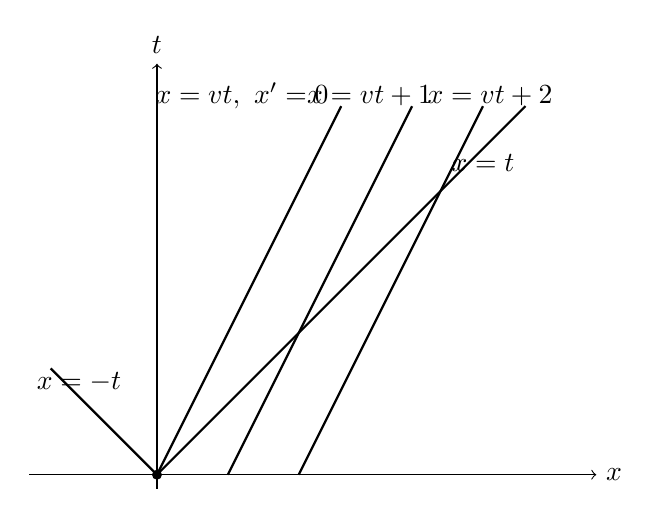
\begin{tikzpicture}[scale=0.9]
\draw[->] (-1.8,0) -- (6.2,0) node[right] {$x$};
\draw[->] (0,-0.2) -- (0,5.8) node[above] {$t$};
\fill (0,0) circle (2pt);
\draw[thick] (0,0) -- (5.2,5.2);
\draw[thick] (0,0) -- (-1.5,1.5);
\draw[thick] (0,0) -- (2.6,5.2);
\draw[thick] (1.0,0) -- (3.6,5.2);
\draw[thick] (2.0,0) -- (4.6,5.2);
\node at (1.2,5.35) {$x=vt,\ x'=0$};
\node at (3.0,5.35) {$x=vt+1$};
\node at (4.7,5.35) {$x=vt+2$};
\node at (4.6,4.4) {$x=t$};
\node at (-1.1,1.3) {$x=-t$};
\end{tikzpicture}
\caption{A clean redraw of the board geometry in relativistic units. Light rays come first, then the family of comoving world lines.}
\end{figure}

Now comes the heart of the construction. Let Fred live on \(x=vt\), Mary on \(x=vt+1\), and Seymour on \(x=vt+2\). We declare the origin to be simultaneous with itself, and then ask which point on Seymour's world line is simultaneous with the origin according to the moving frame. By Einstein's rule, Fred and Seymour must send light signals that reach Mary at the same instant.

\begin{figure}
\centering
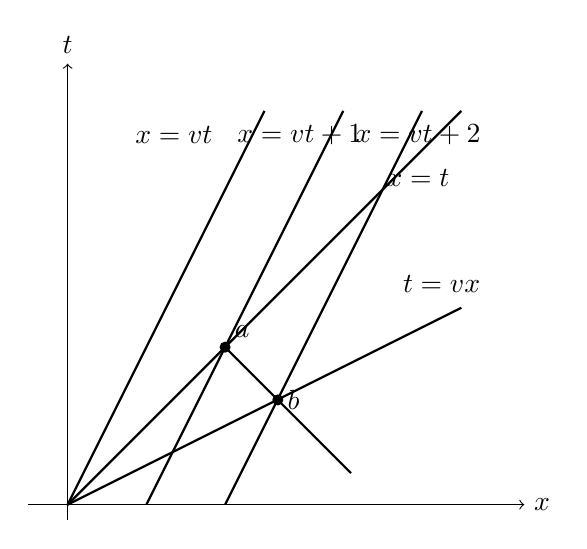
\begin{tikzpicture}[scale=1.0]
\draw[->] (-0.5,0) -- (5.8,0) node[right] {$x$};
\draw[->] (0,-0.2) -- (0,5.6) node[above] {$t$};
\draw[thick] (0,0) -- (5.0,5.0);
\draw[thick] (0,0) -- (2.5,5.0);
\draw[thick] (1.0,0) -- (3.5,5.0);
\draw[thick] (2.0,0) -- (4.5,5.0);
\fill (2,2) circle (2pt);
\fill (2.67,1.33) circle (2pt);
\draw[thick] (2,2) -- (3.6,0.4);
\draw[thick] (0,0) -- (5.0,2.5);
\node[above right] at (2,2) {$a$};
\node[right] at (2.67,1.33) {$b$};
\node at (1.35,4.7) {$x=vt$};
\node at (2.95,4.7) {$x=vt+1$};
\node at (4.45,4.7) {$x=vt+2$};
\node at (4.65,4.7) {};
\node at (4.45,4.15) {$x=t$};
\node at (4.75,2.8) {$t=vx$};
\end{tikzpicture}
\caption{The Fred--Mary--Seymour construction. Point \(a\) lies where Fred's signal reaches Mary; point \(b\) is chosen so Seymour's signal reaches Mary at that same event. The line through the origin and \(b\) is the moving simultaneity line \(t'=0\).}
\end{figure}

The derivation is elementary but important enough to do in detail. Point \(a\) lies at the intersection of
\begin{equation}
x=t
\end{equation}
and
\begin{equation}
x=vt+1.
\end{equation}
Substituting \(x=t\) into the second equation gives
\begin{equation}
t=vt+1,
\end{equation}
and therefore
\begin{equation}
t_a=\frac{1}{1-v},\qquad x_a=\frac{1}{1-v}.
\end{equation}

Next we need the light ray from \(a\) down toward the right. Any \(45^\circ\) line slanting upward to the left satisfies \(x+t=\text{const}\). Evaluating at \(a\) gives
\begin{equation}
x+t=\frac{2}{1-v}
\end{equation}
all along the line \(ab\).

Point \(b\) is the intersection of this line with Seymour's world line:
\begin{equation}
x-vt=2.
\end{equation}
So we solve
\begin{align}
x+t &= \frac{2}{1-v}, \\
x-vt &= 2.
\end{align}
Subtracting the second equation from the first eliminates \(x\):
\begin{equation}
(1+v)t=\frac{2}{1-v}-2=\frac{2v}{1-v}.
\end{equation}
Hence
\begin{equation}
t_B=\frac{2v}{1-v^2}.
\end{equation}
Substituting back gives
\begin{equation}
x_B=\frac{2}{1-v^2}.
\end{equation}
The slope of the line from the origin to \(b\) is therefore
\begin{equation}
\frac{t_B}{x_B}=v.
\end{equation}
So the moving line of simultaneity through the origin is
\begin{equation}
t=vx.
\end{equation}
That is the line \(t'=0\).

This is the lecture's geometric turning point. We now know two things: the moving observer's world line is \(x'=0\), which in the unprimed frame is \(x=vt\), and the moving observer's surface of simultaneity through the origin is \(t'=0\), which in the unprimed frame is \(t=vx\).

\section{From Geometry to Algebra: Deriving the Lorentz Transformation}

Once the geometry has told us where \(x'\) and \(t'\) vanish, the algebra is almost forced.

\begin{figure}
\centering

\includegraphics[width=0.82\textwidth]{lecture_01_figure_06.png}
\caption{The derivation resets from the detailed geometry to the general ansatz \(x'=(x-vt)f(v)\), \(t'=(t-vx)g(v)\).}
\end{figure}

We know that \(x'=0\) whenever \(x=vt\). Therefore \(x'\) must be proportional to \(x-vt\):
\begin{equation}
x'=(x-vt)f(v).
\end{equation}
Likewise, \(t'=0\) whenever \(t=vx\), so
\begin{equation}
t'=(t-vx)g(v).
\end{equation}
At this stage the factors \(f\) and \(g\) are unknown.

Now we use some physics. In the unprimed frame, light moves with unit velocity, so along the right-moving light ray we have \(x=t\). Einstein's postulate says that the same light ray must also satisfy \(x'=t'\) in the moving frame. But when \(x=t\),
\begin{align}
x'&=(1-v)x\,f(v),\\
t'&=(1-v)x\,g(v).
\end{align}
So the only possible choice is
\begin{equation}
f(v)=g(v).
\end{equation}

One ingredient remains. If the primed frame moves with velocity \(v\) relative to the unprimed frame, then the unprimed frame moves with velocity \(-v\) relative to the primed frame. The inverse transformation must therefore have the same shape, with \(v\) reversed in sign:
\begin{equation}
x=(x'+vt')f(v),\qquad t=(t'+vx')f(v).
\end{equation}
Now substitute the direct formulas for \(x'\) and \(t'\) into the inverse expression for \(x\):
\begin{align}
x&=\bigl[(x-vt)+v(t-vx)\bigr]f(v)^2 \\
 &=x(1-v^2)f(v)^2.
\end{align}
This must reduce to \(x=x\), so
\begin{equation}
(1-v^2)f(v)^2=1.
\end{equation}
Therefore
\begin{equation}
f(v)=\frac{1}{\sqrt{1-v^2}}.
\end{equation}
There is also a negative root, but continuity at \(v=0\) fixes the physical choice: when the two frames are not moving relative to each other, we want \(x'=x\), not \(x'=-x\).

We have now derived the Lorentz transformation in relativistic units:
\begin{align}
x'&=\frac{x-vt}{\sqrt{1-v^2}}, \\
t'&=\frac{t-vx}{\sqrt{1-v^2}}.
\end{align}

To restore ordinary units, we use dimensional analysis. The denominator must really involve \(v^2/c^2\), and the term \(vx\) in the time transformation must be replaced by \(vx/c^2\). Thus
\begin{align}
x'&=\frac{x-vt}{\sqrt{1-v^2/c^2}}, \\
t'&=\frac{t-vx/c^2}{\sqrt{1-v^2/c^2}}.
\end{align}
The inverse transformation follows by sending \(v\to -v\):
\begin{align}
x&=\frac{x'+vt'}{\sqrt{1-v^2/c^2}}, \\
t&=\frac{t'+vx'/c^2}{\sqrt{1-v^2/c^2}}.
\end{align}

Only the direction of motion is special. By symmetry,
\begin{equation}
y'=y,\qquad z'=z.
\end{equation}

If \(v\ll c\), then \(v^2/c^2\) is tiny, the square root is essentially \(1\), and the term \(vx/c^2\) is negligible. We recover the Newtonian limit:
\begin{equation}
x'\approx x-vt,\qquad t'\approx t.
\end{equation}

\section{Two Immediate Consequences: Length Contraction and Time Dilation}

Only now, after the transformation has been earned, do we ask what it says about rods and clocks. If we like, we may now introduce the standard shorthand
\begin{equation}
\gamma=\frac{1}{\sqrt{1-v^2/c^2}}.
\end{equation}
But the lecture does not begin with \(\gamma\); it derives the factor first.

\subsection{Length contraction}

Suppose a rod is at rest in the unprimed frame, extending from \(x=0\) to \(x=1\). The moving observer does \emph{not} measure its length by looking at the two ends whenever convenient. The moving observer must look at the two ends at the same primed time. That is the entire point.

\begin{figure}
\centering
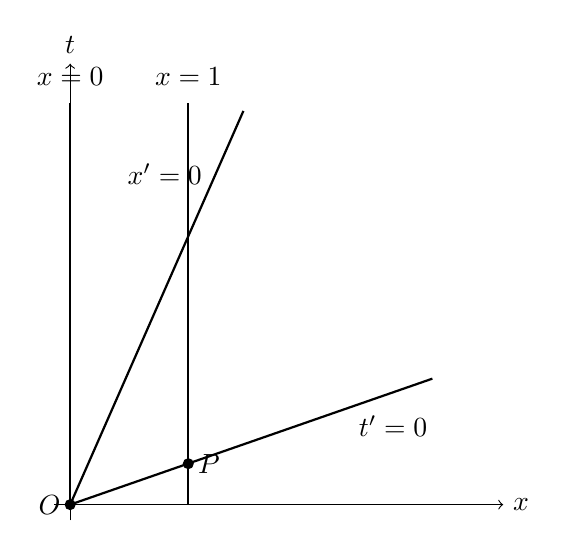
\begin{tikzpicture}[scale=1.0]
\draw[->] (-0.2,0) -- (5.5,0) node[right] {$x$};
\draw[->] (0,-0.2) -- (0,5.6) node[above] {$t$};
\draw[thick] (0,0) -- (0,5.1);
\draw[thick] (1.5,0) -- (1.5,5.1);
\draw[thick] (0,0) -- (2.2,5.0);
\draw[thick] (0,0) -- (4.6,1.6);
\fill (0,0) circle (2pt);
\fill (1.5,0.52) circle (2pt);
\node[left] at (0,0) {$O$};
\node[right] at (1.5,0.52) {$P$};
\node[above] at (0,5.2) {$x=0$};
\node[above] at (1.5,5.2) {$x=1$};
\node at (1.2,4.2) {$x'=0$};
\node at (4.1,1.0) {$t'=0$};
\end{tikzpicture}
\caption{A stationary rod measured in the moving frame. The moving observer measures the separation of the endpoints along the tilted simultaneity line \(t'=0\).}
\end{figure}

At point \(P\), the far end of the rod is at \(x=1\), and the condition \(t'=0\) implies
\begin{equation}
t=vx.
\end{equation}
Therefore at \(P\),
\begin{equation}
t=v.
\end{equation}
In units with \(c=1\), the Lorentz transformation gives
\begin{equation}
x'=\frac{x-vt}{\sqrt{1-v^2}}.
\end{equation}
Substituting \(x=1\) and \(t=v\), we find
\begin{equation}
x'=\frac{1-v^2}{\sqrt{1-v^2}}=\sqrt{1-v^2}.
\end{equation}
So the moving observer assigns length
\begin{equation}
L'=\sqrt{1-v^2}
\end{equation}
to a unit rod. Restoring dimensions,
\begin{equation}
L=L_0\sqrt{1-v^2/c^2}=\frac{L_0}{\gamma}.
\end{equation}

The lecture insists, correctly, that there is no contradiction here. The rest observer measures the distance between one pair of spacetime points; the moving observer measures the distance between a different pair. The difference lies in the different notions of simultaneity.

\subsection{Time dilation}

Now take a clock carried by the moving observer himself. Its world line is \(x'=0\). Ask what the stationary observer says about the passage of time when the moving clock reads \(t'=1\).

\begin{figure}
\centering
\begin{tikzpicture}[scale=1.0]
\draw[->] (-0.2,0) -- (4.2,0) node[right] {$x$};
\draw[->] (0,-0.2) -- (0,5.4) node[above] {$t$};
\draw[thick] (0,0) -- (0,4.8);
\draw[thick] (0,0) -- (1.7,4.2);
\draw[dashed] (1.7,4.2) -- (0,4.2);
\fill (0,0) circle (2pt);
\fill (1.7,4.2) circle (2pt);
\fill (0,4.2) circle (2pt);
\node[left] at (0,0) {$O$};
\node[right] at (1.7,4.2) {$R$};
\node[left] at (0,4.2) {$S$};
\node at (1.3,3.2) {$x'=0$};
\node[above] at (1.7,4.2) {$t'=1$};
\end{tikzpicture}
\caption{A moving clock. The moving observer measures proper time along the slanted world line, while the stationary observer compares with the coordinate time along the vertical axis.}
\end{figure}

Using the inverse transformation in units with \(c=1\),
\begin{equation}
t=\frac{t'+vx'}{\sqrt{1-v^2}},
\end{equation}
and setting \(x'=0\), \(t'=1\), we obtain
\begin{equation}
t=\frac{1}{\sqrt{1-v^2}}.
\end{equation}
So more stationary-frame time elapses than proper time on the moving clock. In general,
\begin{equation}
\Delta t=\gamma\,\Delta t'.
\end{equation}
The moving clock runs slow when judged from the stationary frame.

This is already the seed of the twin paradox. If one twin goes away and comes back, the two twins no longer occupy symmetric inertial frames. The traveler turns around, and that break in inertial symmetry is enough to remove the apparent contradiction. The lecture does not yet develop the full paradox; it merely opens the door.

\subsection{Question \& Answer}

Why is there no contradiction if each observer says the other meter stick is shorter?

Because each observer uses synchronized clocks in \emph{his own} frame, and therefore each observer compares a different pair of spacetime events. The stationary observer measures at fixed \(t\); the moving observer measures at fixed \(t'\). Those are not the same slices of spacetime. The two statements are not competing descriptions of one and the same measurement.

\section{The Invariant Interval, Proper Time, and the Strange Geometry of Spacetime}

The lecture now pivots from coordinate transformations to invariants. This is where spacetime ceases to be merely a bookkeeping device and becomes a geometry of its own.

First recall the Euclidean analogue. If two coordinate systems in the plane are related by a rotation, then although \(x\) and \(y\) change, the combination
\begin{equation}
x'^2+y'^2=x^2+y^2
\end{equation}
does not change. That is the square of the distance from the origin.

One might guess that the spacetime analogue is
\begin{equation}
t'^2+x'^2=t^2+x^2.
\end{equation}
The lecture tries it and rejects it immediately. It is false. But the algebra reveals something better:
\begin{equation}
t'^2-x'^2=t^2-x^2.
\end{equation}
That is the invariant interval in \(1+1\) dimensions. With ordinary units restored, one convenient form is
\begin{equation}
c^2t'^2-x'^2=c^2t^2-x^2.
\end{equation}

\begin{figure}
\centering
\begin{tikzpicture}[scale=1.0]
\draw[->] (-3.0,0) -- (3.8,0) node[right] {$x$};
\draw[->] (0,-0.2) -- (0,4.8) node[above] {$t$};
\draw[thick] (0,0) -- (3.4,3.4);
\draw[thick] (0,0) -- (-3.4,3.4);
\fill (1.1,3.5) circle (2pt);
\fill (2.8,1.4) circle (2pt);
\node[right] at (1.1,3.5) {timelike};
\node[right] at (2.8,1.4) {spacelike};
\node at (2.8,3.0) {$x=t$};
\node at (-2.6,3.0) {$x=-t$};
\end{tikzpicture}
\caption{The light rays \(x=\pm t\) divide spacetime into timelike and spacelike regions. The invariant interval changes sign across the light cone.}
\end{figure}

The sign of the interval matters.

If a point lies on a moving observer's world line, then \(x'=0\), and the invariant reduces to
\begin{equation}
t'^2=t^2-x^2
\end{equation}
in units with \(c=1\). This quantity is the square of the \emph{proper time} along that world line. Restoring dimensions,
\begin{equation}
\tau^2=t^2-\frac{x^2}{c^2}.
\end{equation}
And, as Susskind corrects explicitly near the end of the lecture, proper time itself is the square root:
\begin{equation}
\tau=\sqrt{t^2-\frac{x^2}{c^2}}.
\end{equation}

For a light ray, the interval vanishes:
\begin{equation}
x^2-t^2=0
\qquad\Longleftrightarrow\qquad
x=\pm t
\end{equation}
in units with \(c=1\). So lightlike separation has zero proper time. The lecture phrases this vividly: if a light beam could carry a clock, the clock would not tick.

If
\begin{equation}
t^2-x^2>0,
\end{equation}
the separation is timelike, and the invariant is interpreted as proper time. If instead
\begin{equation}
x^2-t^2>0,
\end{equation}
the separation is spacelike, and one speaks of proper distance rather than proper time. In the spacelike case no physical object moving slower than light can connect the two events.

\subsection{Question \& Answer}

How can the spacetime hypotenuse be shorter than the vertical side, and when does the invariant become proper time rather than proper distance?

The answer to the first part is simply the minus sign. Euclidean geometry teaches us to add squares. Minkowski geometry teaches us that for spacetime the invariant comes from a difference of squares. The minus sign makes the ``hypotenuse'' associated with a moving clock smaller, not larger, than the pure time separation along a vertical world line.

The answer to the second part is causal. If the separation is timelike, so that a subluminal world line can pass from one event to the other, then the invariant gives proper time. If the separation is spacelike, so that no causal trajectory can connect the events, then the invariant is read as proper distance. If the separation is null, a light ray connects the events and the proper time is zero.

The lecture closes with a brief conceptual coda. It is sometimes useful to think of Lorentz transformations as rotations, but they are rotations of a different sort, often described formally as rotations by an imaginary angle. Historically, Susskind emphasizes that Einstein's guiding principle was not merely a correction to Newtonian kinematics but the recognition that Maxwell's equations point to a different symmetry of space and time. Lorentz had related formulas; Einstein turned them into a principle.

\section{Summary}

Special relativity begins here not with a mysterious formula but with a failure. The Galilean rule predicts the wrong speed for light, and the diagnosis is that universal simultaneity must be abandoned. Once simultaneity is defined operationally with light signals, the geometry of the moving frame can be built directly on the \(x\)-\(t\) diagram. From that geometry one derives the Lorentz transformation, then length contraction and time dilation, and finally the invariant interval
\begin{equation}
t'^2-x'^2=t^2-x^2.
\end{equation}
That invariant is the real structural object of the chapter. Coordinates depend on the observer; the interval does not. In the next lecture, this new geometry will be used to understand the motion of particles.